\speakerlabel{Backup}{}

\begin{frame}[t]{\texorpdfstring{\resizebox{0.96\textwidth}{!}{Backup: the learned Black--Scholes hedge matches the analytic curves}}{Backup: the learned Black--Scholes hedge matches the analytic curves}}
  \centering
  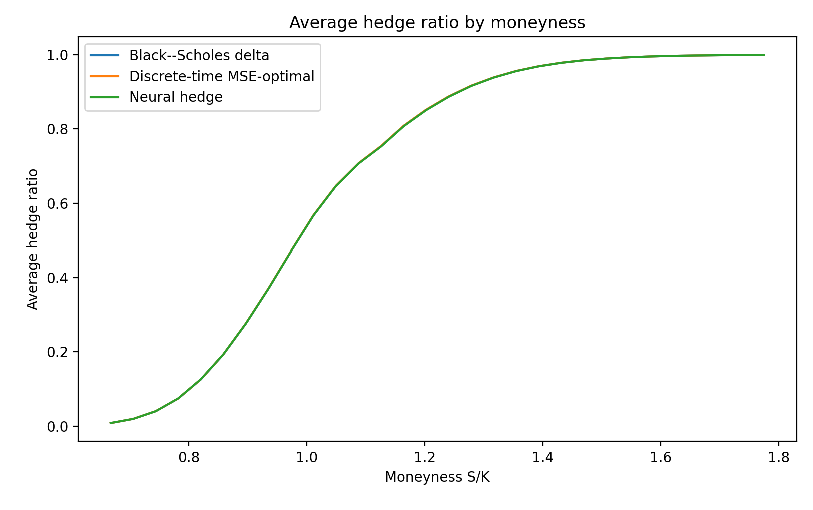
\includegraphics[width=0.94\textwidth,height=5.35cm,keepaspectratio]
    {figures/report_fig_3_3_delta_by_moneyness.pdf}

  \vspace{0.04cm}
  \academicbox[0.92\textwidth]{\centering\small
    The learned hedge ratio closely follows the Black--Scholes delta and
    discrete-time MSE-optimal curves across moneyness.}
  \vspace{-0.04cm}
  \sourcefoot{Submitted report, Figure 3.3 and Sec.\ 3.1.4. Vector crop from the final report.}
\end{frame}

\begin{frame}[t]{\texorpdfstring{\resizebox{0.96\textwidth}{!}{Backup: training and validation losses converge without visible instability}}{Backup: training and validation losses converge without visible instability}}
  \centering
  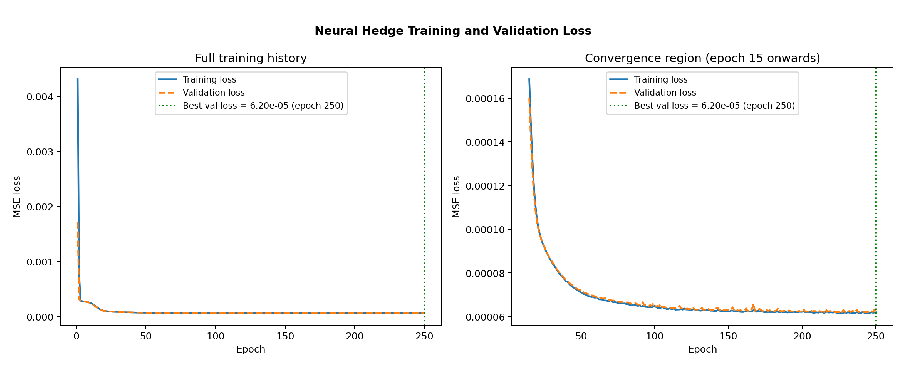
\includegraphics[width=0.98\textwidth,height=5.25cm,keepaspectratio]
    {figures/report_fig_3_6_training_validation_loss.pdf}

  \vspace{0.04cm}
  \academicbox[0.92\textwidth]{\centering\small
    Training and validation losses track closely and flatten late in training;
    the best validation loss occurs at the submitted epoch cap of 250.}
  \vspace{-0.04cm}
  \sourcefoot{Submitted report, Figure 3.6 and Sec.\ 3.1.4. Optimisation and validation evidence, not proof of external generalisation.}
\end{frame}

% Heston/COS oral-defence backups, ordered by the experimental pipeline.

\begin{frame}{State and tensor shapes}
  \centering
  \begin{tikzpicture}[
    box/.style={rounded corners=3pt,draw=DeepNavy!18,fill=Mist,
      minimum height=0.72cm,text width=2.2cm,align=center,font=\scriptsize},
    arr/.style={-{Latex[length=2mm]},color=Teal,line width=0.8pt},
    node distance=0.24cm]
    \node[box] (p) {BS paths\\\((B,N+1)\)};
    \node[box,right=of p] (f) {state stack\\\((B,N,2)\)};
    \node[box,right=of f] (flat) {shared calls\\\((B\!\cdot\!N,2)\)};
    \node[box,right=of flat] (d) {deltas\\\((B,N)\)};
    \node[box,right=of d] (e) {terminal error\\\((B,)\)};
    \draw[arr] (p)--(f);\draw[arr] (f)--(flat);\draw[arr] (flat)--(d);\draw[arr] (d)--(e);
    \node[box,below=0.65cm of p] (hp) {Heston \(S,v,C^h\)\\each \((B,N+1)\)};
    \node[box,right=of hp] (hf) {state stack\\\((B,N,6)\)};
    \node[box,right=of hf] (hflat) {shared calls\\\((B\!\cdot\!N,6)\)};
    \node[box,right=of hflat] (hout) {\((\delta,\eta)\)\\\((B,N,2)\)};
    \node[box,right=of hout] (he) {gain / error\\\((B,)\)};
    \draw[arr] (hp)--(hf);\draw[arr] (hf)--(hflat);\draw[arr] (hflat)--(hout);\draw[arr] (hout)--(he);
  \end{tikzpicture}
  \par\vspace{0.35cm}
  {\scriptsize\color{Slate}The same shared network is applied to every path-date state. Each complete path produces one terminal gain and one terminal hedge error.}
  \sourcefoot{Submitted report, Listings C.1--C.4 and Algorithm A.6.10.}
\end{frame}

\begin{frame}[t]{How gradients accumulate through the shared hedge}
  \centering
  {\fontsize{8.0}{9.1}\selectfont
    \((\delta_{i,n},\eta_{i,n})=f_w(x_{i,n}),\qquad
    L=B^{-1}\sum_{i=1}^B HE_i^2.\)\par}
  \vspace{0.05cm}
  {\fontsize{7.5}{8.6}\selectfont
    \(\displaystyle HE_i=\pi_w+\sum_{n=0}^{N-1}
    [\delta_{i,n}\Delta S_{i,n}+\eta_{i,n}\Delta C^h_{i,n}]-H_i.\)\par}
  \vspace{0.07cm}
  \begin{beamercolorbox}[rounded=true,sep=0.10cm]{block body}
    \centering
    {\fontsize{8.0}{9.3}\selectfont\(
      \boxed{\displaystyle \nabla_wL=\frac{2}{B}\sum_{i=1}^{B}HE_i
      \sum_{n=0}^{N-1}\left[
      \Delta S_{i,n}\nabla_w\delta_{i,n}
      +\Delta C^h_{i,n}\nabla_w\eta_{i,n}\right]}
    \)}
  \end{beamercolorbox}
  \vspace{0.05cm}
  \begin{columns}[T,onlytextwidth]
    \begin{column}{0.40\textwidth}
      \begin{beamercolorbox}[rounded=true,sep=0.10cm]{block body}
        \centering\scriptsize
        \(L\leftarrow HE\leftarrow G_T\leftarrow(\delta,\eta)\leftarrow f_w\leftarrow w\)
      \end{beamercolorbox}
    \end{column}
    \begin{column}{0.56\textwidth}
      {\fontsize{7.5}{8.6}\selectfont\begin{tightitemize}
        \item one weight vector \(w\) is reused at every date;
        \item gradients accumulate across all paths and dates;
        \item no analytic delta or vega labels are supplied;
        \item COS prices are precomputed marks, outside the gradient path.
      \end{tightitemize}}
    \end{column}
  \end{columns}
  \sourcefoot{Submitted report, Sec.\ 2.2.2 and Algorithm A.6.10.}
\end{frame}

\begin{frame}[t]{Heston simulation}
  \begin{columns}[T,onlytextwidth]
    \begin{column}{0.48\textwidth}
      \pill{Correlated shocks}
      {\small\[
        Z_n^S,Z_n^\perp\sim N(0,1),\qquad
        Z_n^v=\rho Z_n^S+\sqrt{1-\rho^2}Z_n^\perp.
      \]}
      \pill[Gold]{Log-Euler stock update}
      {\fontsize{8.3}{9.6}\selectfont\[
        S_{n+1}=S_n\exp\!\left[
        \left(r-\tfrac12v_n^+\right)\Delta t
        +\sqrt{v_n^+\Delta t}\,Z_n^S\right].
      \]}
      {\scriptsize Preserves \(S_{n+1}>0\) and respects multiplicative stock dynamics.}
    \end{column}
    \begin{column}{0.48\textwidth}
      \pill[Coral]{Truncation-based variance update}
      {\fontsize{8.2}{9.5}\selectfont
      \begin{align*}
        \widetilde v_{n+1}&=v_n+\kappa(\theta-v_n^+)\Delta t
        +\xi\sqrt{v_n^+\Delta t}\,Z_n^v,\\
        v_{n+1}&=\max(\widetilde v_{n+1},0),\qquad
        v_n^+=\max(v_n,0).
      \end{align*}}
      {\scriptsize Ordinary Euler--Maruyama can propose negative variance, making the next square root invalid.}
    \end{column}
  \end{columns}
  \vspace{0.08cm}
  \risknote{Standard Monte Carlo generates many paths; log-Euler and full truncation specify each step. This is not an exact Heston transition. Feller positivity does not prevent negative Euler proposals. Discrete paths versus continuous-time COS marks contribute to the small residual COS drift.}
  \sourcefoot{Heston (1993); Lord, Koekkoek \& van Dijk (2010); submitted report, Alg.\ A.3.3 and Listing C.4.}
\end{frame}

\begin{frame}[t]{Two-instrument gain construction}
  \begin{columns}[T,onlytextwidth]
    \begin{column}{0.50\textwidth}
      \pill{Causal state and shared policy}
      {\fontsize{8.0}{9.2}\selectfont\[
        x_n=\left(\log\frac{S_n}{K},\frac{T-t_n}{T},\frac{v_n}{\theta},
        \log\frac{S_n}{K_h},\frac{T_h-t_n}{T_h},\frac{C_n^h}{S_n}\right)
      \]}
      \[
        (\delta_n,\eta_n)=5\tanh\!\bigl(f_w(x_n)\bigr).
      \]
    \end{column}
    \begin{column}{0.46\textwidth}
      \pill[Gold]{Terminal gain and training loss}
      \[
        G_T=\sum_{n=0}^{N-1}\left(\delta_n\Delta S_n+\eta_n\Delta C_n^h\right),
      \]
      \[
        HE=\pi_w+G_T-(S_T-K)^+,
      \]
      \vspace{-0.20cm}
      \[
        L=\mathbb E[HE^2].
      \]
    \end{column}
  \end{columns}
  \vspace{0.12cm}
  \risknote{Executable notebooks and validation outputs were submitted separately; this slide maps the presentation equations to the submitted report algorithms and listings.}
  \sourcefoot{Submitted report, Sec.\ 4.1.4 and Algorithm A.6.10.}
\end{frame}

\begin{frame}[t]{Holdings, trades, and gains}
  \begin{columns}[T,onlytextwidth]
    \begin{column}{0.47\textwidth}
      \pill{Network action: total holdings}
      \begin{beamercolorbox}[rounded=true,sep=0.18cm]{block body}
        \[ (\delta_n,\eta_n)\quad\text{over }[t_n,t_{n+1}]. \]
      \end{beamercolorbox}
      \vspace{0.16cm}
      \pill[Gold]{Trade increments}
      \[
        \Delta\delta_n=\delta_n-\delta_{n-1},\qquad
        \Delta\eta_n=\eta_n-\eta_{n-1}.
      \]
    \end{column}
    \begin{column}{0.49\textwidth}
      \pill{Frictionless one-step gain}
      \begin{beamercolorbox}[rounded=true,sep=0.18cm]{block body}
        \[ \delta_n\Delta S_n+\eta_n\Delta C_n^h. \]
      \end{beamercolorbox}
      \vspace{0.16cm}
      {\small\begin{tightitemize}
        \item the submitted gain equation uses holdings;
        \item trade increments determine transaction costs and turnover;
        \item calling \(\delta_n\) or \(\eta_n\) a trade changes the implementation's meaning.
      \end{tightitemize}}
    \end{column}
  \end{columns}
  \sourcefoot{Submitted report, Sec.\ 4.1.4 and Algorithm A.6.10.}
\end{frame}

\begin{frame}[t]{Why the Heston outputs use scaled tanh}
  \begin{columns}[T,onlytextwidth]
    \begin{column}{0.47\textwidth}
      \pill{Two signed outputs}
      \begin{beamercolorbox}[rounded=true,sep=0.17cm]{block body}
        \centering
        \[ \delta_n=5\tanh(z_{1,n}),\qquad \eta_n=5\tanh(z_{2,n}). \]
        {\color{Teal}\fontsize{17}{19}\selectfont\bfseries \([-5,5]\)\par}
        {\small numerical output range}
      \end{beamercolorbox}
    \end{column}
    \begin{column}{0.49\textwidth}
      \pill[Gold]{Why this map is used}
      \begin{tightitemize}
        \item stock and option holdings can be long or short;
        \item sigmoid's \((0,1)\) range is unsuitable;
        \item scaled tanh permits signed, bounded positions;
        \item the bound improves numerical stability, but is not an optimality theorem.
      \end{tightitemize}
    \end{column}
  \end{columns}
  \vspace{0.18cm}
  \begin{beamercolorbox}[rounded=true,sep=0.13cm]{block body}
    \centering\small Submitted diagnostic: \(\max|\eta^{NN}|\approx1.33\), comfortably below five.
  \end{beamercolorbox}
  \sourcefoot{Submitted report, Sec.\ 4.1.4, Algorithm A.6.10 and Table A.12.}
\end{frame}

\begin{frame}[t]{}
  \vspace*{0.12cm}
  {\color{DeepNavy}\fontsize{18}{21}\selectfont\bfseries Frozen-volatility drift derivation\par}
  \vspace{0.20cm}
  {\scriptsize For the liquid hedge-option proxy \(g(t,S,v)=C_{\bs}(S,K_h,T_h-t,\sqrt v)\):}
  \vspace{0.03cm}
  \centering{\fontsize{8.0}{9.1}\selectfont\(
    (dS)^2=vS^2dt,\quad (dv)^2=\xi^2vdt,\quad dS\,dv=\rho\xi vSdt.
  \)\par}
  \vspace{0.04cm}
  \centering{\fontsize{7.7}{8.9}\selectfont\(
  \begin{aligned}
    dg={}&\Big[g_t+rSg_S+\kappa(\theta-v)g_v+\tfrac12vS^2g_{SS}
      +\tfrac12\xi^2vg_{vv}+\rho\xi vSg_{Sv}\Big]dt\\
      &+g_SS\sqrt v\,dW^S+g_v\xi\sqrt v\,dW^v.
  \end{aligned}
  \)\par}
  \vspace{0.04cm}
  \begin{columns}[T,onlytextwidth]
    \begin{column}{0.46\textwidth}
      \pill[Teal]{Frozen-\(v\) PDE cancellation}
      \centering{\small\(g_t+rSg_S+\tfrac12vS^2g_{SS}-rg=0\)}
    \end{column}
    \begin{column}{0.50\textwidth}
      \pill[Coral]{Residual discounted drift}
      \centering{\small\(\kappa(\theta-v)g_v+\tfrac12\xi^2vg_{vv}+\rho\xi vSg_{Sv}\)}
    \end{column}
  \end{columns}
  \vspace{0.03cm}
  \risknote{At submitted \(r=0\), discounted and undiscounted residuals coincide. The sign is state-dependent; this diagnostic is not a standalone arbitrage proof.}
  \sourcefoot{Submitted report, Sec.\ 4.1.4 and App.\ A.6.3; Black--Scholes (1973); Heston (1993).}
\end{frame}

\begin{frame}[t]{Heston characteristic function used by COS}
  \pill{Conditional transform of log price}
  \begin{beamercolorbox}[rounded=true,sep=0.15cm]{block body}
    {\small\[
      \phi(u;\tau,x,v)=\mathbb E^{\mathbb Q}\!\left[e^{iuX_T}\mid X_t=x,v_t=v\right]
      =\exp\!\left(C(u,\tau)+D(u,\tau)v+iux\right),\qquad X_T=\log S_T.
    \]}
  \end{beamercolorbox}
  \vspace{0.12cm}
  \[
    u_k=\frac{k\pi}{b-a},\qquad k=0,\ldots,N_{\mathrm{COS}}-1.
  \]
  \vspace{0.08cm}
  \begin{columns}[T,onlytextwidth]
    \begin{column}{0.31\textwidth}
      \centering\pill[Teal]{1}\par\small \(\phi\) encodes the conditional distribution in transform space.
    \end{column}
    \begin{column}{0.31\textwidth}
      \centering\pill[Gold]{2}\par\small COS samples \(\phi\) on a deterministic frequency grid.
    \end{column}
    \begin{column}{0.31\textwidth}
      \centering\pill[Coral]{3}\par\small The finite sum gives price, delta and \(\partial C/\partial v\).
    \end{column}
  \end{columns}
  \sourcefoot{Heston (1993); Fang \& Oosterlee (2008); submitted report, Algorithm A.6.6.}
\end{frame}

\begin{frame}[t]{COS pricing}
  \centering{\scriptsize\bfseries Deterministic semi-analytical pricing: no nested Monte Carlo inside COS.\par}
  \vspace{0.04cm}
  \begin{columns}[T,onlytextwidth]
    \begin{column}{0.55\textwidth}
      {\fontsize{8.5}{9.8}\selectfont\[
        \begin{aligned}
        C_{\mathrm{COS}}&\approx e^{-r\tau}
        \sum_{k=0}^{N_{\mathrm{COS}}-1}{}' A_kV_k,\\
        A_k&=\frac{2}{b-a}\Re\!\left[\phi(u_k)e^{-iu_ka}\right],
        \qquad u_k=\frac{k\pi}{b-a}.
        \end{aligned}
      \]}
      {\scriptsize\color{Slate}The prime halves \(k=0\). \(A_k\) is a density coefficient; \(V_k\) is the analytic payoff coefficient. \(u_k\) is the \(k\)-th cosine frequency on \([a,b]\).}
      \vspace{0.08cm}
      \begin{beamercolorbox}[rounded=true,sep=0.09cm]{block body}
        {\scriptsize Heston supplies \(\phi(u)\); COS evaluates the conditional expectation from \(\phi(u_k)\).}
      \end{beamercolorbox}
    \end{column}
    \begin{column}{0.41\textwidth}
      {\small\begin{tightitemize}
        \item \(N_{\mathrm{COS}}=256\), \([a,b]=[-7,7]\);
        \item traded range \(\tau_h\in[0.5,1]\);
        \item Carr--Madan: \(\alpha=1.5\), \(u\in[0,200]\), 20,000 points;
        \item price discrepancy \(5.1\times10^{-8}\);
        \item finite-difference errors: delta \(9.8\times10^{-5}\), variance sensitivity \(4.7\times10^{-4}\).
      \end{tightitemize}}
      \risknote{Validation is local to the submitted traded range.}
    \end{column}
  \end{columns}
  \sourcefoot{Heston (1993); Fang \& Oosterlee (2008); Carr \& Madan (1999); submitted report, Apps.\ A.6.1--A.6.2.}
\end{frame}

\begin{frame}[t]{Analytic Heston stock-and-option hedge}
  \centering{\fontsize{7.7}{8.8}\selectfont\(
  \begin{aligned}
    dC^T&=\cdots+\Delta^T S\sqrt v\,dW^S+V^T\xi\sqrt v\,dW^v,\\
    d(\delta S+\eta C^h)&=\cdots+(\delta+\eta\Delta^h)S\sqrt v\,dW^S
      +\eta V^h\xi\sqrt v\,dW^v.
  \end{aligned}
  \)\par}
  \vspace{0.05cm}
  \begin{beamercolorbox}[rounded=true,sep=0.09cm]{block body}
    \centering
    {\small Match \(\eta V^h=V^T\) and \(\delta+\eta\Delta^h=\Delta^T\):\quad
    \(\displaystyle\boxed{\eta=\frac{V^T}{V^h},\qquad\delta=\Delta^T-\eta\Delta^h}\)}
  \end{beamercolorbox}
  \vspace{0.04cm}
  \begin{columns}[T,onlytextwidth]
    \begin{column}{0.48\textwidth}
      \pill{Heston COS delta--variance benchmark}
      {\small Heston COS supplies target and liquid hedge-option sensitivities.}
    \end{column}
    \begin{column}{0.48\textwidth}
      \pill[Gold]{BS-proxy Greek heuristic on the COS option path}
      {\small Frozen-\(v\) BS sensitivities set positions; gains use the same COS marks.}
    \end{column}
  \end{columns}
  \vspace{0.04cm}
  \risknote{Local continuous-time first-order diffusion matching; not the finite-grid terminal-MSE optimum. The report table retains “delta--vega”, although \(V=\partial C/\partial v\).}
  \sourcefoot{Submitted report, Sec.\ 4.1.4 and Algorithms A.6.8--A.6.9.}
\end{frame}

\begin{frame}[t]{\large Pricing accuracy and finite-grid hedge optimality are different questions}
  \begin{columns}[T,onlytextwidth]
    \begin{column}{0.47\textwidth}
      \pill{What COS establishes}
      \begin{tightitemize}
        \item model-consistent Heston option prices;
        \item independently validated prices and sensitivities;
        \item local first-order exposures for the COS Greek rule.
      \end{tightitemize}
    \end{column}
    \begin{column}{0.49\textwidth}
      \pill[Coral]{What it does not optimise}
      \begin{tightitemize}
        \item finite-grid terminal MSE;
        \item between-date gamma and variance curvature;
        \item spot--variance cross effects and changing Greeks.
      \end{tightitemize}
    \end{column}
  \end{columns}
  \vspace{0.16cm}
  \begin{beamercolorbox}[rounded=true,sep=0.16cm]{block body}
    \small Model misspecification may accidentally compensate for finite-grid effects in this tested parameter regime. That ordering does \textbf{not} imply that Black--Scholes is a better Heston pricer.
  \end{beamercolorbox}
  \vspace{0.12cm}
  {\small The neural policy trains directly on terminal MSE. Turnover is supporting diagnostic evidence, not proof of the ordering.}
  \sourcefoot{Submitted report, Sec.\ 4.1.4 and Tables 4.5--4.6.}
\end{frame}

\begin{frame}[t]{Fair-premium centring}
  \begin{columns}[T,onlytextwidth]
    \begin{column}{0.55\textwidth}
      \begin{beamercolorbox}[rounded=true,sep=0.12cm]{block body}
        {\fontsize{8.1}{9.4}\selectfont\[
          \boxed{\pi_j^*=\arg\min_\pi\mathbb E_{\mathrm{test}}
          \!\left[(\pi+G_T^j-H)^2\right]
          =\mathbb E_{\mathrm{test}}[H-G_T^j]}
        \]}
        \vspace{-0.12cm}
        \[ HE_j=\pi_j^*+G_T^j-H,\qquad \mathbb E_{\mathrm{test}}[HE_j]=0. \]
      \end{beamercolorbox}
      {\scriptsize\begin{tightitemize}
        \item applied separately to every headline strategy;
        \item removes test-sample mean error;
        \item RMSE compares centred dispersion; Loss CVaR95 compares centred downside tail risk;
        \item not used during training: the NN jointly learns a raw premium and hedge weights.
      \end{tightitemize}}
    \end{column}
    \begin{column}{0.41\textwidth}
      \pill{Data roles remain separate}
      {\small
      \begin{tabular}{@{}p{0.27\linewidth}p{0.61\linewidth}@{}}
        \toprule
        Training & Fit weights and learned premium\\
        Validation & Select architecture / best epoch\\
        Test & Final fair-centred comparison\\
        \bottomrule
      \end{tabular}}
      \vspace{0.12cm}
      \risknote{Because \(\pi_j^*\) is estimated on the same test paths as the metrics, this is not fully out-of-sample joint pricing and hedging.}
    \end{column}
  \end{columns}
  \sourcefoot{Submitted report, Sec.\ 4.1.4, Tables 4.5--4.6 and A.11, and Algorithm A.6.10.}
\end{frame}

\begin{frame}[t]{Three-seed Heston comparison}
  \centering\pill[Gold]{Comparator: BS-proxy Greek heuristic on the COS option path}
  \vspace{0.10cm}
  \begin{table}
    \centering\small
    \begin{tabular}{cS[table-format=1.6]S[table-format=1.6]S[table-format=2.1]S[table-format=2.1]}
      \toprule
      Seed & {NN RMSE} & {Heuristic RMSE} & {RMSE imp.\ (\%)} & {CVaR95 imp.\ (\%)}\\
      \midrule
      111 & 0.007806 & 0.009838 & 20.6 & 26.3\\
      222 & 0.007715 & 0.009871 & 21.8 & 27.0\\
      333 & 0.007346 & 0.009864 & 25.5 & 28.0\\
      \midrule
      \multicolumn{3}{r}{Mean pairwise improvement} & \bfseries 22.7 & \bfseries 27.1\\
      \bottomrule
    \end{tabular}
  \end{table}
  \vspace{0.10cm}
  {\scriptsize\begin{tightitemize}
    \item The three-seed cell retrained the stock-only tanh and stock-plus-option NNs and reevaluated the COS delta--variance and BS-proxy Greek analytic rules on each fresh test set.
    \item No hedge, BS-proxy stock delta and representative-only rows in the main table were not part of this four-strategy rerun.
  \end{tightitemize}}
  \vspace{0.04cm}
  \risknote{Three seeds demonstrate consistency across submitted runs; they do not support high-powered confidence intervals.}
  \sourcefoot{Submitted report, Table A.11.}
\end{frame}

\begin{frame}[t]{Observable-information robustness}
  \begin{columns}[T,onlytextwidth]
    \begin{column}{0.47\textwidth}
      \pill{Causal variance proxy}
      \begin{tightitemize}
        \item EWMA decay \(\lambda=0.94\);
        \item \(\operatorname{corr}(\hat v_t,v_t)=0.777613\);
        \item relative variance-proxy RMSE \(=0.369375\).
      \end{tightitemize}
    \end{column}
    \begin{column}{0.49\textwidth}
      \pill[Gold]{Submitted mean RMSE}
      \begin{table}
        \centering\fontsize{8.4}{9.8}\selectfont
        \begin{tabular}{lS[table-format=1.6]}
          \toprule Strategy & {RMSE}\\ \midrule
          Stock-plus-option NN & 0.007877\\
          \shortstack[l]{BS-proxy Greek heuristic on\\the COS option path} & 0.010734\\
          \bottomrule
        \end{tabular}
      \end{table}
    \end{column}
  \end{columns}
  \vspace{0.10cm}
  \begin{beamercolorbox}[rounded=true,sep=0.12cm]{block body}
    {\small The EWMA state is a causal compressed history of past squared returns; the MLP itself remains non-recurrent.}
  \end{beamercolorbox}
  \vspace{0.08cm}
  \risknote{\(C_t^h/S_t\) remains contemporaneously observable and variance-informative, so this is not a stock-return-only filtering experiment.}
  \sourcefoot{Submitted report, Sec.\ 4.1.4 and Tables A.10, A.12, A.15; J.P. Morgan/Reuters (1996).}
\end{frame}

\begin{frame}[t]{Why the hedge option differs from the target}
  \begin{columns}[T,onlytextwidth]
    \begin{column}{0.47\textwidth}
      \pill{Target liability}
      \begin{beamercolorbox}[rounded=true,sep=0.18cm]{block body}
        \centering\Large\bfseries \(K=0.9,\quad T=0.5\)
      \end{beamercolorbox}
    \end{column}
    \begin{column}{0.49\textwidth}
      \pill[Gold]{Liquid hedging option}
      \begin{beamercolorbox}[rounded=true,sep=0.18cm]{block body}
        \centering\Large\bfseries \(K_h=1,\quad T_h=1\)
      \end{beamercolorbox}
    \end{column}
  \end{columns}
  \vspace{0.18cm}
  \begin{tightitemize}
    \item near-ATM options generally have useful variance sensitivity;
    \item \(T_h>T\) keeps the liquid hedging option alive throughout the target horizon;
    \item trading an identical target option would largely trivialise the problem;
    \item the target liability need not itself be a liquid traded contract.
  \end{tightitemize}
  \sourcefoot{Submitted report, Sec.\ 4.1.4 and the target/hedge-option configuration.}
\end{frame}

\begin{frame}[t]{What the martingale diagnostic measures}
  \begin{columns}[T,onlytextwidth]
    \begin{column}{0.52\textwidth}
      \pill{Sample mean over \([0,T]\)}
      \begin{beamercolorbox}[rounded=true,sep=0.15cm]{block body}
        \[ \widehat m=\frac1M\sum_{i=1}^M\left(C_T^{h,(i)}-C_0^h\right). \]
      \end{beamercolorbox}
      \vspace{0.15cm}
      \pill[Gold]{Monte Carlo standard error}
      \[ \widehat{\mathrm{SE}}(\widehat m)=\frac{s(C_T^h-C_0^h)}{\sqrt M}. \]
    \end{column}
    \begin{column}{0.44\textwidth}
      {\small\begin{tightitemize}
        \item individual paths fluctuate; the statistic concerns average movement;
        \item under \(r=0\), the reference is zero;
        \item the target horizon ends at \(T=0.5<T_h=1\);
        \item this diagnoses dynamic inconsistency, not standalone executable arbitrage.
      \end{tightitemize}}
    \end{column}
  \end{columns}
  \vspace{0.03cm}
  \risknote{Proxy: \(-0.009482\) (SE \(0.000459\)); COS: \(-0.000118\) (SE \(0.000479\)). The COS residual is negligible, not exactly zero.}
  \sourcefoot{Submitted report, Table A.9 and Algorithm A.6.8.}
\end{frame}

\begin{frame}[t]{Backup: the discrete-time conditional projection}
  \centering{\fontsize{7.7}{8.9}\selectfont\(
  \begin{aligned}
    \min_{\pi,\delta}\quad&\mathbb{E}\!\left[\left(\pi+\sum_{j=0}^{N-1}\delta_j\Delta S_j-H\right)^2\right],\\
    0={}&\mathbb{E}\!\left[\left(H-\pi-\sum_{j=0}^{N-1}\delta_j\Delta S_j\right)
      \Delta S_n\mid\mathcal{F}_{t_n}\right].
  \end{aligned}
  \)\par}
  \vspace{0.12cm}
  {\small Under submitted \(r=0\), \(S\) is a martingale, so\par}
  \vspace{0.06cm}
  \centering{\fontsize{7.7}{8.9}\selectfont\(
    \displaystyle
    \deltadt_n=\frac{\mathbb E[H\Delta S_n\mid\mathcal F_{t_n}]}
    {\mathbb E[(\Delta S_n)^2\mid\mathcal F_{t_n}]}
    =\frac{\operatorname{Cov}(H,\Delta S_n\mid S_{t_n})}
    {\operatorname{Var}(\Delta S_n\mid S_{t_n})}.
  \)\par}
  \vspace{0.08cm}
  \risknote{This simplification is tied to the submitted \(r=0\) martingale setting; local and global quadratic hedges need not coincide more generally.}
  \sourcefoot{Submitted report, Appendix A.4; Schweizer (1995, 2001).}
\end{frame}


\begin{frame}{Backup: method-to-code map}
  \scriptsize
  \begin{tabular}{@{}p{0.21\textwidth}p{0.24\textwidth}p{0.22\textwidth}p{0.18\textwidth}@{}}
    \toprule
    Mathematical concept & Displayed implementation & Report evidence & Primary expert\\
    \midrule
    Exact BS path simulation & \texttt{simulate\_gbm\_paths} & Listing C.1; Alg.\ A.3.1 & Micaela / Glasson\\
    Self-financing terminal error & \texttt{hedge\_error} & Listing C.2; Alg.\ A.6.1 & Micaela / Glasson\\
    Shared Markov hedge & \texttt{SharedMarkovHedge} & Listing C.3; Sec.\ 2.2.2 & Kaiden / Micaela\\
    Heston full-truncation simulation & PyTorch loop in Listing C.4 & Listing C.4; Alg.\ A.3.3 & Glasson / Siphelele\\
    COS liquid-option pricing & Algorithms A.6.6--A.6.8 & App.\ A.6.1--A.6.2 & Glasson\\
    Two-instrument neural gain & Algorithm A.6.10 & Sec.\ 4.1.4 & Siphelele / Glasson\\
    \bottomrule
  \end{tabular}
  \vspace{0.25cm}
  \risknote{Executable notebooks and validation outputs were submitted separately; this slide maps the presentation equations to the submitted report algorithms and listings.}
\end{frame}


\begin{frame}{Backup: transaction costs change the learned policy}
  \[
    V_T^\lambda
    =\pi+\sum_{n=0}^{N-1}\delta_n\Delta S_n
    -\lambda\sum_{n=0}^{N-1}S_{t_n}\lvert\delta_n-\delta_{n-1}\rvert,
    \qquad \delta_{-1}=0.
  \]
  \begin{table}
    \centering
    \scriptsize
    \begin{tabular}{c l S[table-format=1.6]S[table-format=1.6]S[table-format=1.6]}
      \toprule
      \(\lambda\) & Strategy & {RMSE} & {Loss CVaR95} & {Turnover}\\
      \midrule
      0.0025 & BS cost-adjusted & 0.008492 & 0.021464 & 4.497364\\
      0.0025 & Cost-aware NN & 0.008077 & 0.018694 & 4.386880\\
      0.0050 & BS cost-adjusted & 0.010013 & 0.025565 & 4.497364\\
      0.0050 & Cost-aware NN & 0.008331 & 0.019269 & 4.284602\\
      \bottomrule
    \end{tabular}
  \end{table}
  \risknote{Comparator is a cost-adjusted frictionless delta, not a full optimal-cost benchmark such as Leland or Whalley--Wilmott.}
  \sourcefoot{Submitted report, Appendix A.7 and Table A.16.}
\end{frame}

\begin{frame}{Backup: data-generation comparison}
  \begin{table}
    \centering
    \scriptsize
    \begin{tabular}{r l S[table-format=1.6]S[table-format=1.6]}
      \toprule
      Paths & Method & {RMSE} & {Loss CVaR95}\\
      \midrule
      10,000 & Crude MC & 0.009430 & 0.021266\\
      10,000 & LHS & 0.009201 & 0.020845\\
      10,000 & Sobol + Brownian bridge & 0.009174 & 0.020865\\
      \midrule
      100,000 & Crude MC & 0.007865 & 0.018218\\
      100,000 & LHS & 0.007846 & 0.018331\\
      100,000 & Sobol + Brownian bridge & 0.007840 & 0.018125\\
      \bottomrule
    \end{tabular}
  \end{table}
  \vspace{0.22cm}
  \claimbox{At 10,000 paths, structured methods reduce RMSE by roughly 2.4--2.7\%; by 100,000 paths the difference is negligible.}
  \sourcefoot{Submitted report, Sec.\ 3.1.5 and Tables A.7--A.8.}
\end{frame}

\begin{frame}{Backup: experimental protocol}
  \scriptsize
  \begin{tabular}{p{0.26\textwidth}rrrrp{0.24\textwidth}}
    \toprule
    Experiment & Train & Val & Test & Batch & Training / seeds\\
    \midrule
    Architecture selection & 100k & 20k & 50k & 256 & 60 epochs; 2026--2028\\
    Final BS benchmark & 100k & 30k & 100k & 4096 & 250 epochs; base 123\\
    Parameter robustness & 50k & 15k & 50k & 4096 & 150 epochs\\
    Conditioned hedger & 200k & 30k & 50k / case & 4096 & 250 epochs; 777\\
    Heston stock + option & 100k & 25k & 100k & 4096 & 150 epochs; base 123\\
    \bottomrule
  \end{tabular}
  \vspace{0.28cm}
  \begin{tightitemize}
    \item Adam learning rate \(10^{-3}\) unless otherwise stated.
    \item Baseline: \(S_0=1,K=0.9,T=0.5,r=0,\sigma=0.4,N=125\).
    \item Architecture search uses more updates per epoch via batch size 256; final experiments use 4096.
  \end{tightitemize}
  \sourcefoot{Submitted report, Appendix A.1, Table A.1.}
\end{frame}

\begin{frame}{Backup: AI assistance and verification}
  \small
  \begin{tabular}{p{0.41\textwidth}p{0.49\textwidth}}
    \toprule
    Assistance area disclosed & Human verification reported\\
    \midrule
    Code drafting and debugging & Executed notebooks, code inspection and exported results\\
    Mathematical explanations and LaTeX & Checked against theory and cited sources\\
    Report organisation and consistency & Tables checked against CSV/TeX outputs and figures\\
    COS implementation support & Independent Carr--Madan Fourier price check\\
    Neural experiment support & BS analytic and finite-grid benchmarks; archived outputs\\
    Documentation and reproducibility & Checklists, packaging review and author decisions\\
    \bottomrule
  \end{tabular}
  \vspace{0.24cm}
  \risknote{The report names ChatGPT and Claude. It states that AI suggestions were not authoritative and that all final methodological and interpretive decisions remained with the authors.}
  \sourcefoot{Submitted report, Appendix B.}
\end{frame}

\begin{frame}{{\fontsize{15}{18}\selectfont Backup: architecture selection by seed}}
  \begin{table}
    \centering
    \small
    \begin{tabular}{c l S[table-format=1.3e-1]S[table-format=1.6]}
      \toprule
      Seed & Validation winner & {Val.\ loss} & {Test RMSE}\\
      \midrule
      2026 & Shared norm.\ \(64{\times}3\), tanh & 6.025e-5 & 0.007883\\
      2027 & Shared norm.\ \(64{\times}3\), tanh & 6.164e-5 & 0.007916\\
      2028 & Shared norm.\ \(64{\times}2\), ReLU & 6.014e-5 & 0.007855\\
      \bottomrule
    \end{tabular}
  \end{table}
  \vspace{0.25cm}
  \claimbox{The \(64{\times}3\) tanh model won two seeds and had the best mean validation loss and test RMSE; the ReLU alternative was close.}
  \sourcefoot{Submitted report, Tables A.3--A.6.}
\end{frame}

\begin{frame}[allowframebreaks]{Backup: references}
  \scriptsize
  \nocite{blackscholes1973,merton1973,buehler2019,heston1993,fang2008,carrmadan1999,
    schweizer1995,schweizer2001,follmerschweizer1991,lord2010,leland1985,
    whalley1997,glasserman2004,gatheral2006,rufwang2020,kingmaba2015,riskmetrics1996}
  \bibliographystyle{plainnat}
  \bibliography{references}
\end{frame}
